\section{解決策}

\begin{frame}
  \center
  \huge{解決策}
\end{frame}

\begin{frame}
  \frametitle{環境識別子(EC)を利用したスコープ表現\tiny{[Sudo+2014]}}
  % \begin{center}
  %   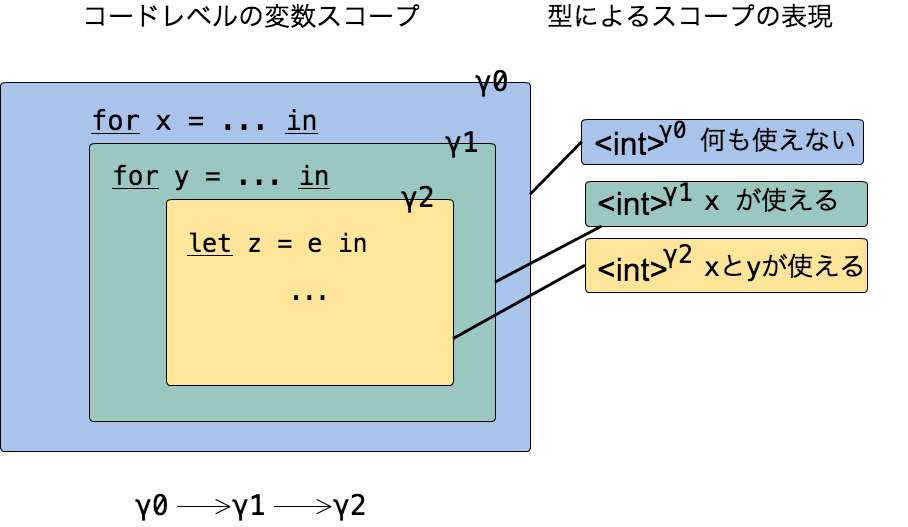
\includegraphics[clip,height=5.7cm]{./img/ec_for.png}
  % \end{center}
  % \begin{flushright}
  %   $\gamma_i ... \text{Refined Environment Classifier}$
  % \end{flushright}

  \newcommand\ml{\multicolumn}
  \center
  {\Large
    \begin{tabular}{l|l|l|l|l|l|}
      \cline{2-6}
      \alert{$\mathbf \gamma0$} & \ml{5}{|l|}{$\cfordo{x = e1}{e2}~~~~~~~~~~~~~~~$} \\ \cline{3-5}
                                & \alert{$\mathbf \gamma1$} & \ml{3}{|l|}{$\cfordo{y = e3}{e4}$} & \\ \cline{4-4}
                                &           & \alert{$\mathbf \gamma2$} & \ml{1}{|l|}{$\caryset{a}{(x,y)} cc$} & ~~ & \\ \cline{4-4}
                                &           & \ml{3}{|l|}{\ }    &               \\ \cline{3-5}
                                & \ml{5}{|l|}{~~~~~~~~~~~~~~~~~~ } \\ \cline{2-6}
    \end{tabular}
  }

  \begin{center}
    \begin{tabular}{c|c}
      スコープ & 使えるコード変数 \\ \hline
      \red{$\gamma0$} & なし \\ \hline
      \red{$\gamma1$} & $x$ \\ \hline
      \red{$\gamma2$} & $x, y$
    \end{tabular}\qquad
  \end{center}

  \red{$\gamma2$} $\ord$ \red{$\gamma1$} $\ord$ \red{$\gamma0$}
\end{frame}

% \begin{frame}
%   \frametitle{環境識別子(EC)を利用したスコープ表現\tiny{[Sudo+2014]}}
%   % 大なり記号はスコープの大きさを表しているのではなく,使える自由変数の集合の大きさを表している
%   型システムでコード変数のスコープを表現:

%   \center
%   \begin{align*}
%     & \Gamma = \gamma2 \ord \gamma1,~
%       x : \codeTs{\textbf{int}}{\gamma1},~
%       y : \codeTs{\textbf{int}}{\gamma2}
%   \end{align*}

%   \begin{tabular}{c|c}
%     $\gamma1$ & $\gamma2$ \\ \hline \hline
%     \uncover<1->{$\Gamma ~\vdash~ x : \codeTs{\textbf{int}}{\gamma1}~~ \alert{\text{OK}}$} & \uncover<1->{$\Gamma ~\vdash~ x : \codeTs{\textbf{int}}{\gamma2}~~ \alert{\text{OK}}$} \\ \hline

%     \uncover<1->{$\Gamma ~\vdash~ y : \codeTs{\textbf{int}}{\gamma1}~~ \alert{\text{NG}}$} & \uncover<1->{$\Gamma ~\vdash~ y : \codeTs{\textbf{int}}{\gamma2}~~ \alert{\text{OK}}$} \\ \hline

%     \uncover<1->{$\Gamma ~\vdash~ x\cPlus y : \codeTs{\textbf{int}}{\gamma1}~~  \alert{\text{NG}}$} & \uncover<1->{$\Gamma ~\vdash~ x\cPlus y : \codeTs{\textbf{int}}{\gamma2}~~  \alert{\text{OK}}$}
%   \end{tabular}

%   \bigskip

%   \begin{uncoverenv}<2->
%     コードレベルのラムダ抽象の型付け規則で固有変数条件を利用:

%     \[
%       \infer[(\gamma_2~\text{is eigen var})]
%       {\Gamma \vdash \cfun{x}{e} : \codeTs{t_1\to t_2}{\gamma_1} }
%       {\Gamma,~\gamma_2 \ord \gamma_1,~x:\codeTs{t_1}{\gamma_2} \vdash
%         e : \codeTs{t_2}{\gamma_2}}
%     \]
%   \end{uncoverenv}
% \end{frame}

\begin{frame}
  \frametitle{環境識別子(EC)を利用したスコープ表現}

  先行研究:
  \begin{itemize}
  \item 局所的なスコープをもつ破壊的変数をもつコード生成の体系に対する(型安全な)型システムの構築
    [Sudo,Kiselyov,Kameyama 2014]
  \item グローバルなスコープをもつ破壊的変数への拡張
    [Kiselyov,Kameyama,Sudo 2016]
  \item[◯] コントロールオペレータには非対応
  \end{itemize}

  \medskip
  \begin{uncoverenv}<2->
    \begin{exampleblock}{問題点:}
      shift0/reset0 などのコントロールオペレータは,スコープの包含関係を逆転させてしまう.
    \end{exampleblock}
  \end{uncoverenv}
\end{frame}


% \begin{frame}
%   \frametitle{本研究の解決策}
%   \flushleft
%   
\includegraphics[clip,height=3cm]{./img/ecgraph.png}
%   \begin{itemize}
%   \item<2-> $\gamma1$ のコード変数は $\gamma2$ では使ってはいけない
%   \item<2-> $\gamma2$ のコード変数は $\gamma1$ では使ってはいけない
%   \item<3->[$\Rightarrow$] \red{$\gamma1$ と $\gamma2$ の間に順序を付けない}
%   \end{itemize}

%   \begin{itemize}
%   \item<4-> $\gamma1, \gamma2$ のコード変数は $\gamma3$ で使ってよい
%   \item<5->[$\Rightarrow$] \red{Sudoらの体系に $\cup$ (ユニオン) を追加} % ジョイン
%   \end{itemize}
% \end{frame}

\begin{frame}[fragile]
  \frametitle{コード生成+shift0/reset0 の型システム\small{ (の一部)}}
  reset0:
  \[
    \infer{\Gamma \vdash \resetz{e} : \codeTs{t}{\gamma} ~;~ \sigma}
    {\Gamma \vdash e : \codeTs{t}{\gamma} ~;~ \codeTs{t}{\gamma}, \sigma}
  \]

  shift0:
  \[
    \infer{\Gamma \vdash \shiftz{k}{e} : \codeTs{t1}{\red{\gamma1}} ~;~ \codeTs{t0}{\gamma0},\sigma}
    {\Gamma,~k:\contT{\codeTs{t1}{\gamma1}}{\codeTs{t0}{\gamma0}}
      \vdash e : \codeTs{t0}{\red{\gamma0}} ~;~ \sigma
      & \Gamma \models \gamma1 \ord \gamma0
    }
  \]

  throw:
  \[
    \infer
    {\Gamma,~k:\contT{\codeTs{t1}{\gamma1}}{\codeTs{t0}{\gamma0}}
      \vdash \throw{k}{v} : \codeTs{t0}{\gamma2} ~;~ \sigma}
    {\Gamma
      \vdash v : \codeTs{t1}{\red{\gamma1 \cup \gamma2}} ~;~ \sigma
      & \Gamma \models \gamma2 \ord \gamma0
    }
  \]
\end{frame}


%%% Local Variables:
%%% mode: latex
%%% TeX-master: "slide_oishi"
%%% End:
